\documentclass{beamer}
\usepackage{csquotes}
\usepackage{tikz}
\usetikzlibrary{arrows,positioning,shapes.geometric, calc}
\usepackage{amsmath}
\usepackage{listings, xcolor}
\usepackage{lmodern}
\usepackage{adjustbox}
\usepackage{booktabs}
\usepackage{colortbl}
\usepackage{caption}
\usepackage{icomma}
\usepackage{bigstrut}
\usepackage{geometry}
\usepackage{subfigure}


\DeclareMathOperator*{\argmin}{argmin}

\usetheme{metropolis}           % Use metropolis theme
\title{$L_0$-norm and Large Scale Genetic Machine Learning}
\date{\today}
\author{Robert M. Porsch}
\institute{Center of Genomic Science}
\begin{document}
\maketitle

\begin{frame}[t]{Introduction}
  I have two objectives:
  \begin{itemize}
    \item Introduce $L_0$ for penalized regressions
    \item Data engineering for machine learning on genetic data
  \end{itemize}
  Literature used:\\
  Learning Sparse Neural Networks through $L_0$ Regularization \\
  \emph{Louizos, Max Kingma} \\
  \vspace{0.5cm}
  The Variational Garrote \\
  \emph{Kappen,  Gomez}
\end{frame}

\begin{frame}[t]{Penalized Regression}
  Let $\mathcal{D}$ the dataset consisting of $N$ input-output pairs $\{(x_1, y_1), \ldots, (x_N, y_N)\}$ and consider the following regularized minimization procedure

  \begin{equation} 
    \mathcal{R}(\theta) = \frac{1}{N} ( \sum^N_{i=1} \mathcal{L}(h(x_i; \theta), y_i)) + \lambda\mathcal{P}(\theta)
  \end{equation}

  With $\theta^* = \underset{\theta}{\argmin}\{\mathcal{R}(\theta)\}$.

  $\mathcal{P}(\theta)$ is a penalization function for the parameters $\theta$.
\end{frame}

\begin{frame}[t]{Forms of $\mathcal{P}(\theta)$}
  $L_1$-norm:
  \begin{equation}
    \mathcal{P}_{L_1}(\theta) = ||\theta||_1 = \sum^{|\theta|}_{i=1} |\theta_i|
  \end{equation}
  or $L_2$-norm:
  \begin{equation}
    \mathcal{P}_{L_2}(\theta) = ||\theta||_2 =  \sum^{|\theta|}_{i=1} \theta_i^2
  \end{equation}
  When being more general. Let $p \geq 1$
  \begin{equation}
    \mathcal{P}_{L_p}(\theta) = ||\theta||_p = (\sum^{|\theta|}_{i=1} |\theta_i|^{p})^{1/p}
  \end{equation}
\end{frame}

\begin{frame}[t]{What about $p=0$?}
  There are \textbf{two} $L_0$-norms:
  \begin{itemize}
    \item $L_0$-norm (Established by Banach and not relevant here)
    \item $L_0$-`norm' (Established by David Donoho)
  \end{itemize}
  The $\L_0$-`norm' is not a real norm, we just call it because it is the limit of the $L_p$ norm:
  \begin{equation}
    \matcal{P}_{L_0}(\theta) = ||\theta||_0 = \lim_{p \rightarrow 0} (\sum^{|\theta|}_{i=1} |\theta_i|^{p})^{1/p}
  \end{equation}
  In general we define it as 
  \begin{equation}
    \matcal{P}_{L_0}(\theta) = ||\theta||_0 = \sum^{|\theta|}_{j=1} \mathcal{I}[\theta_j \neq 0]
  \end{equation}
  So its just the count of non-zero parameters.
\end{frame}

\begin{frame}[t]{Some graphical representation always helps}
  \begin{figure}[htpb]
    \centering
    \includegraphics[width=0.8\linewidth]{norms.png}
    \caption{Various Norms}\label{fig:norms}
  \end{figure} 
  Furthermore, 
  \begin{itemize}
    \item same as the other norms, it encourages sparsity in the parameters
    \item $L_0$ does induce any shrinkage in the parameters
  \end{itemize}
\end{frame}

\begin{frame}[t]{There is a problem however \ldots}
  Optimization is computationally intractable under the $L_0$ penalty,
  \begin{itemize}
    \item non-differentiable %TODO check this again
    \item $2^{|\theta|}$ possible states
    \item NP-hard problem
  \end{itemize}
  So there is a need to relax the discrete nature of $L_0$ to allow for efficient optimizations.
\end{frame}

\begin{frame}[t]{The General Recipe}
  The first step is to reformulate the $L_0$ norm under the parameters $\theta$.
  Hence let,
  \begin{equation}
    \begin{matrix}
      \theta_j = \tilde{\theta_j}z_j, & z_j \in \{0, 1\}, & \tilde{\theta}_j \neq 0
    \end{matrix}
  \end{equation}
  Therefore $z_j$ can be considered as binary gates (parameter has an effect).

  Then we can reformulate the minimization from Eq. 1 by letting $q(z_j|\pi_j) = Bern(\pi_j)$
  \begin{equation}
    \mathcal{R}(\tilde{\theta}, \pi) = \mathbb{E}_{q(z|\pi)} [\frac{1}{N} ( \sum^N_{i=1} \mathcal{L}(h(x_i; \tilde{\theta} \otimes z), y_i)] + \lambda \sum^{|\theta|}_{j=1} \pi_j
  \end{equation}
  with  $\tilde{\theta}^*, \pi^* = \underset{{\tilde{\theta}, \pi}}{\argmin} \{\mathcal{R}(\tilde{\theta}, \pi)\}$

  However, the discrete nature of $z$ makes it still difficult to minimize $\pi$.
  A solution is to give $z$ a \textbf{hard-sigmoid} function.
\end{frame}

\begin{frame}[t]{Hard-sigmoid function}
  \small
  Let s be a continuous random variable with a distribution $q(s)$ with parameter $\phi$.
  Then we can give the gates $z$ a hard sigmoid function with:
  \begin{equation}
    \begin{align*}
      s \sim& q(s|\phi) \\
      z =& \min(1, \max(0, s))
    \end{align*}
  \end{equation}
  Then the probability of the gates being non-zero is
  \begin{equation}
    q(z \neq 0 | \delata) =  1 - Q(s\leq 0 | \phi)
  \end{equation}
  in which $Q(\cdot)$ is the cumulative distribution function of s
  \begin{equation}
    \begin{split}
      \mathcal{R}(\tilde{\theta}, \phi) = \mathbb{E}_{q(s|\phi)} [\frac{1}{N} ( \sum^N_{i=1} \mathcal{L}(h(x_i; \tilde{\theta} \otimes g(s)), y_i)] + \\ 
      \lambda \sum^{|\theta|}_{j=1} (1 - Q(s_j \leq 0 | \phi_j))
    \end{split}
  \end{equation}
  with $\theta^*, \phi^* = \underset{{\tilde{\theta}, \phi}}{\argmin} \{\mathcal{R}(\tilde{\theta}, \phi)\}$ and $g(\cdot) = \min(1, \max(0, \cdot))$
\end{frame}

\begin{frame}[t]{Some graphical help}
  \begin{figure}[htpb]
    \centering
    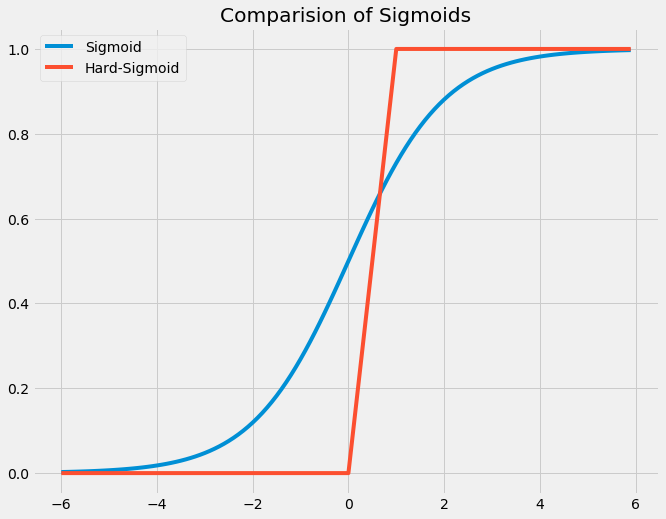
\includegraphics[width=0.5\linewidth]{sigmoids.png}
    \caption{Sigmoid functions}\label{fig:sigmoids}
  \end{figure} 
  However, we still need to chose a function $q(s)$.
\end{frame}

\begin{frame}[t]{The Hard Concrete Distribution}
  The literature suggests to use a hard concrete distribution as a smoothing function $q(s)$. 
  The parameters of the distribution are $\phi = (\log \alpha, \beta)$ and can be stretched to $(\gamma, \zeta)$ intervals.
  \begin{equation}
    \begin{align*}
      u \sim \mathcal{U}(0,1) \\
      s = Sigmoid((\log u - \log(1-u) + \log\alpha)/\beta) \\
      \bar{s} = s(\zeta - \gamma) + \gamma 
    \end{align*}
  \end{equation}
  \begin{figure}[htpb]
    \centering
    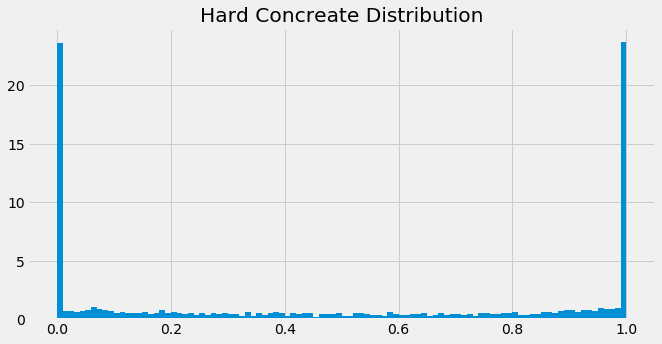
\includegraphics[width=0.5\linewidth]{hard_concrete.png}
    \caption{Sample from the Hard Concrete Distribution}\label{fig:hard_concrete}
  \end{figure} 
\end{frame}

\section{Implementation and Plumbing}

\begin{frame}[t]{Implementation}
  Use of stochastic gradient descent (SGD) with Pytorch.
  \begin{itemize}
    \item Not as optimal as coordinated descent, but reasonably fast
    \item Pytorch implementation was easier than tensorflow
    \item Works fine on test data
  \end{itemize}
  \textbf{Challenge:} \\
  The plumbing (data engineering)
  \\
  \begin{itemize}
    \item Process of the UKB in parallel efficiently
    \item Hail is limited in its flexibility
    \item Currently using Dask on our cluster
  \end{itemize}
\end{frame}

\begin{frame}[t]{Task processing}
  \begin{figure}[htpb]
    \centering
    \includegraphics[width=0.8\linewidth]{Dask_processing.png}
  \end{figure} 
\end{frame}

\begin{frame}[t]{Using Dask}
  Dask lets you specify each task in a lazy fashion (computation is done when you need it).
  \begin{figure}[htpb]
    \centering
    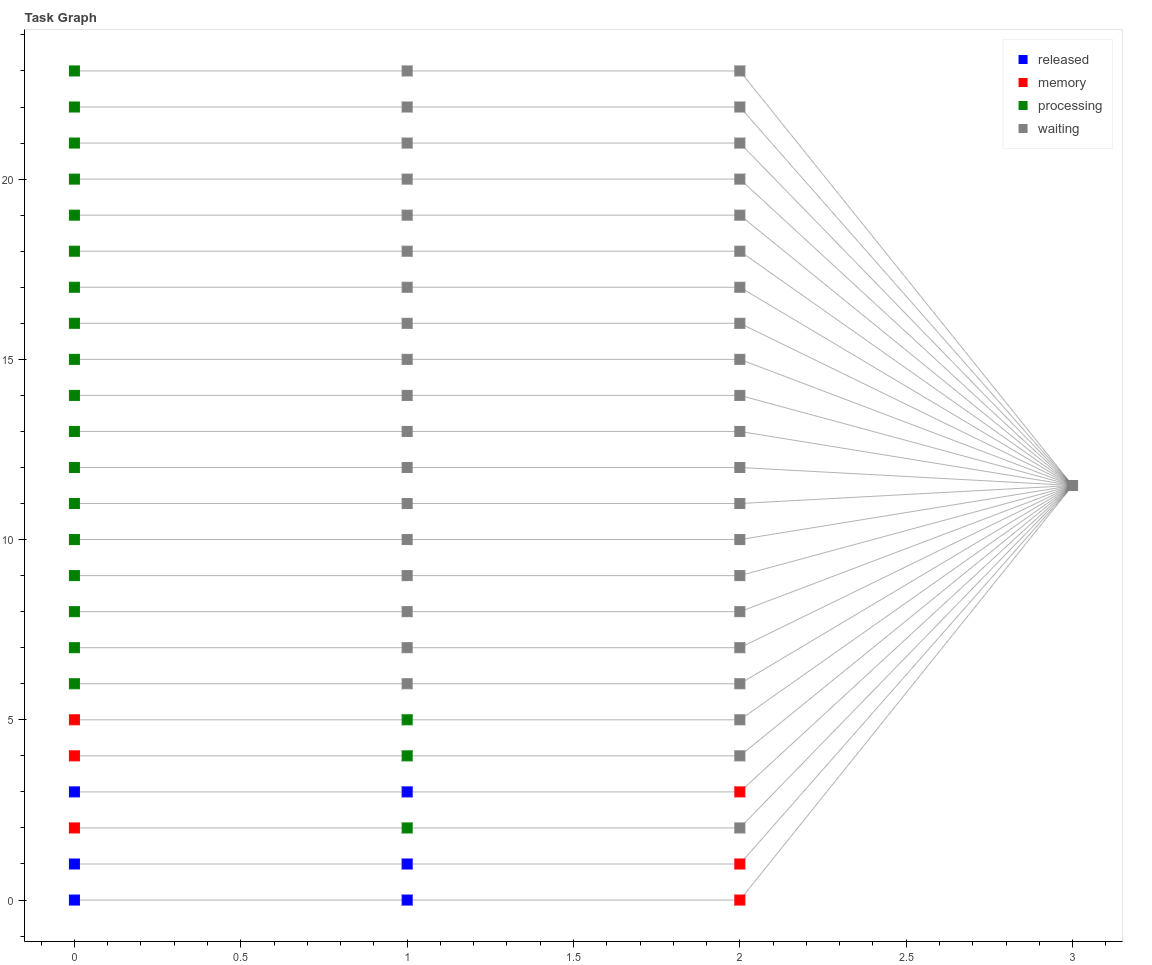
\includegraphics[width=0.7\linewidth]{task_plot.png}
  \end{figure} 
\end{frame}

\begin{frame}[t]{Some Results}
 \textbf{In process}  
\end{frame}
\end{document}
